% !TeX program = pdflatex
% Part V of the godsil-gutman-lean series.
% Counting Trees Without Listing Them — a machine-checked proof of Kirchhoff's
% matrix-tree theorem in Lean 4.
% Build: pdflatex matrix-tree-lean.tex  (twice, for refs)
% Verified against the Lean source 2026-06-10 (lake build, 3074 jobs, exit 0;
% #print axioms SimpleGraph.det_reducedLapMatrix_eq_card_spanningTrees ->
% propext, Classical.choice, Quot.sound only). Toolchain v4.30.0-rc2, local Mathlib.

\documentclass[11pt]{article}
\usepackage[T1]{fontenc}
\usepackage{lmodern}
\usepackage{amsmath,amssymb,amsthm,booktabs,graphicx,hyperref}
\usepackage{xurl}
\usepackage[table]{xcolor}
\definecolor{ggteal}{HTML}{1B6F8C}
\definecolor{ggband}{HTML}{DCE7EB}
\definecolor{ggamber}{HTML}{E08A1E}
\usepackage[margin=1in]{geometry}
\usepackage{microtype}
\usepackage[most]{tcolorbox}
\usepackage{tikz}
\usetikzlibrary{arrows.meta,positioning}
\setlength{\emergencystretch}{2em}
\graphicspath{{figures/}}
\newtheorem{theorem}{Theorem}
\newtheorem{lemma}{Lemma}
\newtheorem{definition}{Definition}
\newcommand{\lean}[1]{\texttt{#1}}
\newcommand{\Z}{\mathbb{Z}}
\newcommand{\R}{\mathbb{R}}
\newcommand{\N}{\mathbb{N}}
\DeclareMathOperator{\dist}{dist}
\hypersetup{colorlinks=true,linkcolor=ggteal,citecolor=ggteal,urlcolor=ggteal}
\newtcbox{\keybox}{on line,boxrule=0.9pt,colframe=ggteal,colback=ggband!40,
  arc=3pt,left=8pt,right=8pt,top=5pt,bottom=5pt}
\newcommand{\keyeq}[1]{\begin{center}\keybox{$\displaystyle #1$}\end{center}}

\title{\bf Counting Trees Without Listing Them\\[4pt]
  \large\normalfont A machine-checked proof of Kirchhoff's matrix-tree theorem in Lean~4}
\author{Carles Mar\'in\thanks{Formalized with AI assistance (Claude, Anthropic); the mathematics
and all claims are the author's responsibility. The methodology is discussed in
Section~\ref{sec:implications}.}\\[3pt]
  \normalsize Independent researcher\\
  \normalsize \texttt{karlesmarin@gmail.com}}
\date{June 2026}

\begin{document}
\maketitle

\begin{abstract}
I present a machine-checked, \lean{sorry}-free proof, in Lean~4 over Mathlib, of
\emph{Kirchhoff's matrix-tree theorem}: over any integral domain, the determinant of the reduced
Laplacian of a finite simple graph equals its number of spanning trees. The proof is assembled
from four formalized pieces, each of independent use: the Cauchy--Binet formula for
$\det(AB)$ of a rectangular pair; the \emph{oriented} incidence matrix and its Gram factorization
$NN^{\mathsf T}=D-A$ (Mathlib has only the unoriented incidence matrix, whose Gram matrix is
$D+A$); the Cauchy--Binet expansion of the reduced Laplacian determinant into a sum of squared
maximal minors; and a dichotomy theorem identifying the squared minor as $1$ exactly on the edge
sets of spanning trees and $0$ elsewhere. The dichotomy is proved \emph{without} the textbook
leaf-deletion induction: each non-root vertex of a connected subgraph is assigned its
\emph{parent edge} on a geodesic to the root, the resulting recolumned minor is upper-triangular
under the lexicographic key $(\text{distance to root},\,\text{vertex})$, and the determinant is
the product of its $\pm1$ diagonal. A by-product of the design is that no separate acyclicity
argument is ever constructed: connectivity and the edge count---which together, classically,
already characterize trees---are the only inputs the formal proof consumes. The headline theorem depends only on the three
standard axioms. I am exact about the boundary: the result is for finite simple graphs over an
integral domain; the weighted Kirchhoff polynomial, the all-minors theorem and the directed
version are mapped but not built; an independent Lean formalization of Cauchy--Binet (not in
Mathlib) appeared in the Grinberg-textbook project and is discussed in
Section~\ref{sec:boundary}; for the matrix-tree theorem itself I was unable to locate a prior
formalization in any proof assistant, though such a claim can only ever be made to the best of
one's knowledge.
\end{abstract}

\noindent\emph{Reader's map.} If you read only one thing, read Theorem~\ref{thm:kirchhoff} and
Figure~\ref{fig:triangular}---the statement, and the picture of why a spanning tree's minor is
$\pm1$. The proof is a single chain (Figure~\ref{fig:road}); every link has its own section,
a figure or a worked table, and an example small enough to check by hand. The honest limits are in
Section~\ref{sec:boundary}.

\begin{figure}[h]
\centering
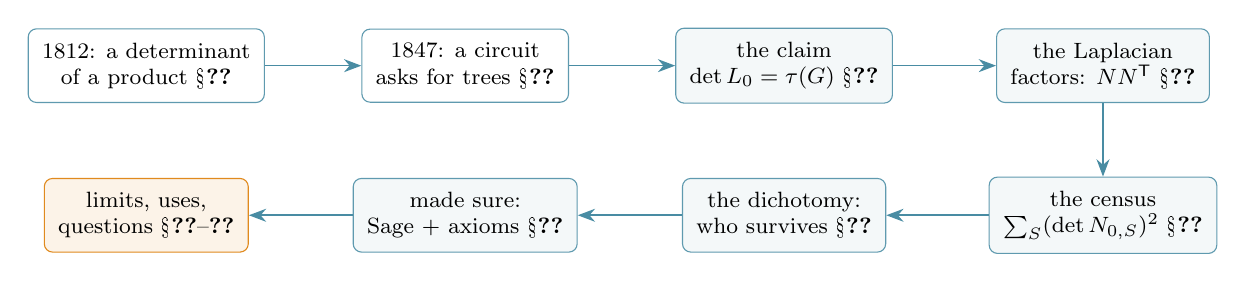
\begin{tikzpicture}[
  theme/.style={draw=ggteal!70,fill=ggband!30,rounded corners=3pt,align=center,
    inner sep=5pt,font=\footnotesize,minimum height=9mm},
  hist/.style={draw=ggteal!70,fill=white,rounded corners=3pt,align=center,
    inner sep=5pt,font=\footnotesize,minimum height=9mm},
  last/.style={draw=ggamber,fill=ggamber!10,rounded corners=3pt,align=center,
    inner sep=5pt,font=\footnotesize,minimum height=9mm},
  flow/.style={-{Stealth[length=2.2mm]},semithick,ggteal!80}]
  \node[hist]  (a) at (0,1.5)    {1812: a determinant\\of a product\ \S\ref{sec:cb}};
  \node[hist]  (b) at (4.05,1.5) {1847: a circuit\\asks for trees\ \S\ref{sec:intro}};
  \node[theme] (c) at (8.1,1.5)  {the claim\\$\det L_0=\tau(G)$\ \S\ref{sec:result}};
  \node[theme] (d) at (12.15,1.5){the Laplacian\\factors: $NN^{\mathsf T}$\ \S\ref{sec:gram}};
  \node[theme] (e) at (12.15,-0.4){the census\\$\sum_S(\det N_{0,S})^2$\ \S\ref{sec:sum}};
  \node[theme] (f) at (8.1,-0.4) {the dichotomy:\\who survives\ \S\ref{sec:dichotomy}};
  \node[theme] (g) at (4.05,-0.4){made sure:\\Sage + axioms\ \S\ref{sec:verification}};
  \node[last]  (h) at (0,-0.4)   {limits, uses,\\questions\ \S\ref{sec:boundary}--\ref{sec:questions}};
  \draw[flow] (a) -- (b);
  \draw[flow] (b) -- (c);
  \draw[flow] (c) -- (d);
  \draw[flow] (d) -- (e);
  \draw[flow] (e) -- (f);
  \draw[flow] (f) -- (g);
  \draw[flow] (g) -- (h);
\end{tikzpicture}
\caption{The reader's map: the themes of the paper in their logical order---two classical
ingredients, the claim, the factorization that decomposes it, the census, the decision, the
checks, and what remains.}
\label{fig:readermap}
\end{figure}


% ---------------------------------------------------------------
\section{Introduction: two memoirs and a circuit}
\label{sec:intro}

On the 30th of November, 1812, two memoirs on determinants were read at the Institut de France
on the same day: one by Jacques Binet, one by Augustin-Louis Cauchy~\cite{Binet1812,Cauchy1812}.
Both contained, among much else, the formula now bearing both names: the determinant of a
product of two rectangular matrices is a sum, over all ways of selecting a square from the
shared dimension, of products of corresponding minors. It is the earliest theorem in this paper,
and the deepest single ingredient.

Thirty-five years later, Gustav Kirchhoff was not studying determinants. He was studying
electrical circuits---the linear equations governing currents in a resistor
network~\cite{Kirchhoff1847}---and found that the common denominator of their solution, the
determinant that Cramer's rule places under every current, counts something purely
combinatorial: the spanning trees of the network's graph. In modern dress, with
$D$ the diagonal of vertex degrees and $A$ the adjacency matrix, the \emph{Laplacian} $L=D-A$ of
a graph $G$ on $n$ vertices is singular (its rows sum to zero), but striking any one row and the
matching column leaves an $(n-1)\times(n-1)$ matrix $L_0$ with
\[
  \det L_0 \;=\; \tau(G),
\]
the number of spanning trees of $G$---whichever row was struck. A determinant computable in
polynomial time counts a family that is typically exponential; the matrix knows the answer
without anyone listing a single tree.

The theorem then led a double life. Borchardt, in 1860, was the first to obtain the
labelled-tree count $n^{n-2}$ by evaluating a determinant~\cite{Borchardt1860}; Cayley's short
note of 1889, which gave the formula its name and credits Borchardt, exhibits the count that
the matrix-tree determinant produces on the complete graph~\cite{Cayley1889}. In 1940,
Brooks, Smith, Stone and Tutte dissected rectangles into squares by interpreting the dissection
as a current flowing through a planar network---Kirchhoff's circuits returning to
mathematics~\cite{BSST1940}. Tutte extended the count to directed graphs and
arborescences~\cite{Tutte1948}; Chaiken and Kleitman proved the all-minors
generalization~\cite{ChaikenKleitman1978,Chaiken1982}. In modern probability the theorem is
load-bearing: Wilson's algorithm samples a uniform spanning tree faster than the cover
time~\cite{Wilson1996}, the transfer-current theorem makes the uniform spanning tree a
determinantal process~\cite{BurtonPemantle1993}, and effective resistances---ratios of spanning
tree counts---drive spectral sparsification~\cite{SpielmanSrivastava2011}. The standard accounts
are~\cite{Moon1970,Biggs1993,GodsilRoyle,StanleyEC2,LyonsPeres}.

What the theorem did not have, as far as I could find, is a machine-checked proof. The Lean
mathematical library~\cite{Mathlib} has the Laplacian matrix and knows its kernel; it has the
\emph{unoriented} incidence matrix; it recently gained, in an independent textbook-formalization
project, the Cauchy--Binet formula~\cite{Grinberg,FaabianRepo}---but not the matrix-tree theorem,
and I found no formalization of it in Isabelle's Archive of Formal Proofs or in the Coq/Rocq
ecosystem either. This paper closes that gap, as Part~V of a series formalizing the
walk--matching--spectrum circle of ideas around the matching
polynomial~\cite{PartI,PartII,Bass,PartIII,PartIV}.

One more thing, and it is the twist this paper sets down. Every textbook proof of the dichotomy
at the heart of the theorem---\emph{a set of $n-1$ edges has minor $\pm1$ if it is a spanning
tree and $0$ otherwise}---peels a leaf and inducts. The formal proof here does something a
machine finds far more comfortable: it \emph{sorts}. Each non-root vertex is matched to its
\emph{parent edge} on a geodesic toward the root; ordering vertices by distance makes the minor
upper-triangular with $\pm1$ diagonal, and the determinant falls out as a product
(Figure~\ref{fig:triangular}). No induction on graphs anywhere. A smaller observation, of
proof engineering rather than mathematics: of the two halves of the tree characterization
``connected and acyclic with $n-1$ edges'', the formal proof only ever consumes connectivity
plus the count---the equivalent acyclicity half, though of course implied, never has to be
materialized as a lemma. The machine is never asked to look for a cycle.

% ---------------------------------------------------------------
\section{The result}
\label{sec:result}

Throughout, $G$ is a finite simple graph on a vertex type $V$ with a linear order (any
enumeration of the vertices), $v_0\in V$ a fixed \emph{root}, and $R$ a commutative ring---an
integral domain where stated. Write $n=|V|$. The Lean statement of the headline theorem is:

\begin{theorem}[{\lean{SimpleGraph.det\_reducedLapMatrix\_eq\_card\_spanningTrees}}]
\label{thm:kirchhoff}
Let $R$ be an integral domain. Then
\keyeq{\det L_0 \;=\; \#\Bigl\{\,S\subseteq\mathrm{Sym}^2 V \;:\; |S|=n-1,\;
S\subseteq E(G),\; (V,S)\ \text{is a tree}\,\Bigr\}}
where $L_0$ is the Laplacian of $G$ with the row and column of $v_0$ deleted, and the count is
cast into $R$.
\end{theorem}

In Lean the right-hand side is a \lean{Finset.filter} over the subtype of
$(n-1)$-element subsets of \lean{Sym2 V}, the condition being
$\uparrow\!S\subseteq G.\lean{edgeSet}\;\wedge\;(\lean{fromEdgeSet}\ \uparrow\!S).\lean{IsTree}$;
since \lean{fromEdgeSet} places the subgraph on \emph{all} of $V$, \lean{IsTree} already
encodes spanning. Every spanning tree of $G$ has exactly $n-1$ edges and is determined by its
edge set, so the filter counts spanning trees, each exactly once.

\begin{figure}[t]
  \centering
  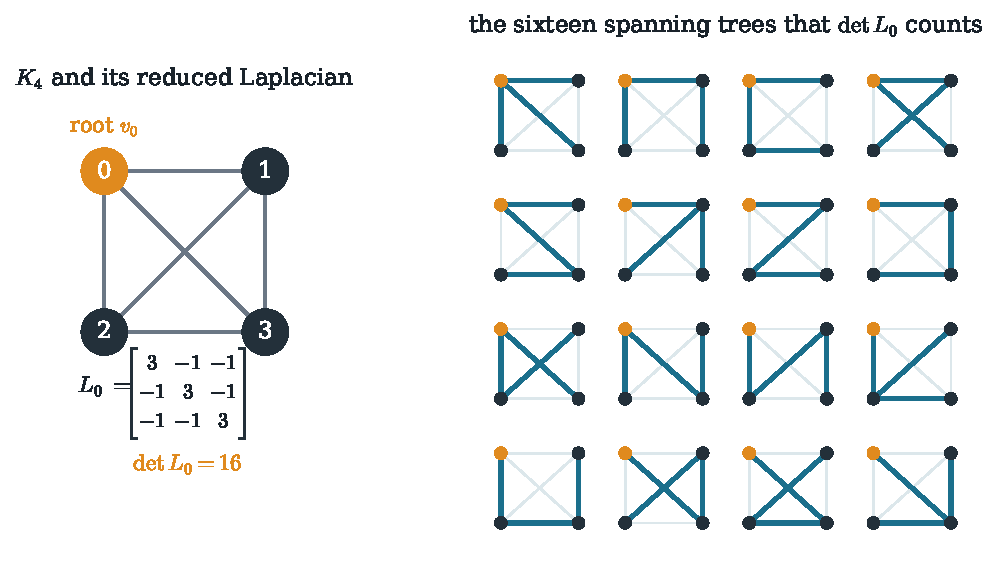
\includegraphics[width=0.96\textwidth]{mt_fig1_k4trees}
  \caption{The theorem on $K_4$, rooted at $v_0$. The reduced Laplacian is the $3\times3$
  matrix on the left; its determinant is $16$, and on the right are the sixteen spanning trees
  it counts. Cayley's formula $n^{n-2}$ gives $4^2=16$; the determinant arrives at the same
  number without enumerating anything.}
  \label{fig:k4}
\end{figure}

What is the theorem \emph{for}? It converts an exponential enumeration into a polynomial-time
linear-algebra computation. The Petersen graph has $2000$ spanning trees; nobody finds them by
listing. One writes down the $9\times9$ reduced Laplacian and takes a determinant. The same
trade powers everything in Section~\ref{sec:implications}: reliability counts, uniform sampling,
effective resistances. Table~\ref{tab:numbers} shows the theorem in action on six classical
graphs, with both sides computed independently in SageMath.

\begin{table}[h]
\centering
\rowcolors{2}{ggband!35}{white}
\begin{tabular}{lccc}
\toprule
\rowcolor{ggteal!18} graph & $n$ & $\det L_0$ & $\tau(G)$ (independent count) \\
\midrule
$K_4$        & 4  & 16   & 16   \\
$K_5$        & 5  & 125  & 125  \\
$C_6$ (cycle)& 6  & 6    & 6    \\
$K_{3,3}$    & 6  & 81   & 81   \\
$Q_3$ (cube) & 8  & 384  & 384  \\
Petersen     & 10 & 2000 & 2000 \\
\bottomrule
\end{tabular}
\caption{Both sides of Theorem~\ref{thm:kirchhoff} computed independently (SageMath,
exact integer arithmetic). Note $K_4$ and $K_5$ are Cayley's $4^{2}$ and $5^{3}$; $C_6$ counts
its six single-edge deletions.}
\label{tab:numbers}
\end{table}

% ---------------------------------------------------------------
\section{The chain in four stones}
\label{sec:chain}

The formal proof is a chain of four results, each usable on its own. Figure~\ref{fig:road} shows
the dependencies; Table~\ref{tab:loadbearing} lists the Lean names. The narrative of the next
four sections simply walks the chain.

\begin{figure}[h]
\centering
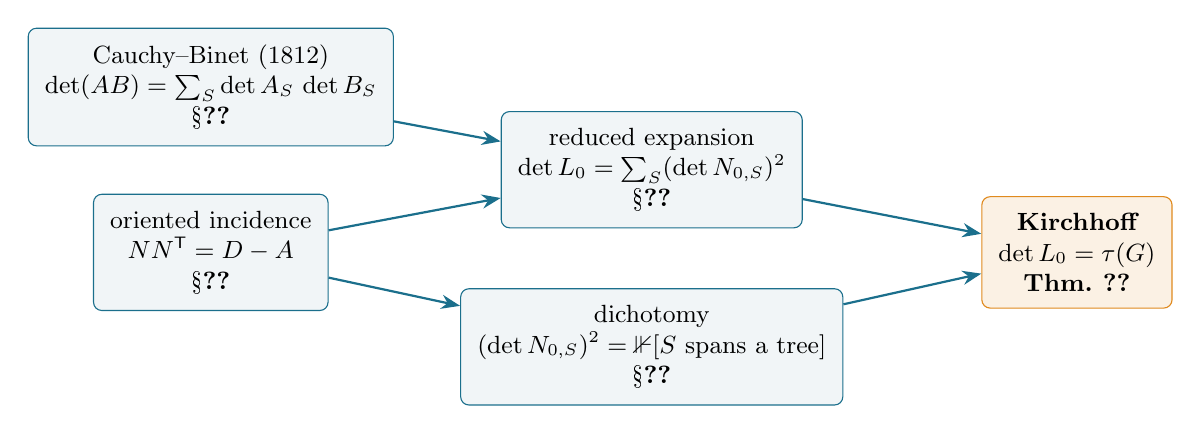
\begin{tikzpicture}[
  stone/.style={draw=ggteal,fill=ggband!40,rounded corners=3pt,align=center,
    inner sep=6pt,font=\small},
  final/.style={draw=ggamber,fill=ggamber!12,rounded corners=3pt,align=center,
    inner sep=6pt,font=\small\bfseries},
  arr/.style={-{Stealth[length=2.4mm]},thick,ggteal}]
  \node[stone] (cb) at (0,2.1) {Cauchy--Binet (1812)\\
    $\det(AB)=\sum_S \det A_S\,\det B_S$\\ \S\ref{sec:cb}};
  \node[stone] (gram) at (0,0) {oriented incidence\\
    $NN^{\mathsf T}=D-A$\\ \S\ref{sec:gram}};
  \node[stone] (sum) at (5.6,1.05) {reduced expansion\\
    $\det L_0=\sum_S(\det N_{0,S})^2$\\ \S\ref{sec:sum}};
  \node[stone] (dich) at (5.6,-1.2) {dichotomy\\
    $(\det N_{0,S})^2=\mathbb 1[S\ \text{spans a tree}]$\\ \S\ref{sec:dichotomy}};
  \node[final] (kir) at (11.0,0) {Kirchhoff\\ $\det L_0=\tau(G)$\\
    Thm.~\ref{thm:kirchhoff}};
  \draw[arr] (cb) -- (sum);
  \draw[arr] (gram) -- (sum);
  \draw[arr] (sum) -- (kir);
  \draw[arr] (dich) -- (kir);
  \draw[arr] (gram) -- (dich);
\end{tikzpicture}
\caption{The proof chain. Two classical ingredients combine into the sum-of-squares expansion;
the dichotomy decides each summand; the count falls out.}
\label{fig:road}
\end{figure}

\begin{table}[h]
\centering\footnotesize
\rowcolors{2}{ggband!35}{white}
\begin{tabular}{lll}
\toprule
\rowcolor{ggteal!18} Lean theorem & statement & file (under \lean{Ihara/}) \\
\midrule
\lean{det\_mul\_cauchyBinet} & $\det(AB)=\sum_S\det A_S\det B_S$ & \lean{CauchyBinet.lean} \\
\lean{orientedIncMatrix\_mul\_transpose} & $NN^{\mathsf T}=D-A$ & \lean{OrientedIncidence.lean} \\
\lean{det\_reducedLapMatrix\_eq\_sum\_sq} & $\det L_0=\sum_S(\det N_{0,S})^2$ & \lean{MatrixTree.lean} \\
\lean{sq\_det\_minor\_eq\_ite} & $(\det N_{0,S})^2=\mathbb 1[S\ \text{spans a tree}]$ & \lean{SpanningTreeMinor.lean} \\
\lean{det\_reducedLapMatrix\_eq\_card\_spanningTrees} & $\det L_0=\tau(G)$ & \lean{Kirchhoff.lean} \\
\bottomrule
\end{tabular}
\caption{The load-bearing results. All are \lean{sorry}-free; each
\lean{\#print axioms} reports exactly \lean{propext}, \lean{Classical.choice},
\lean{Quot.sound}.}
\label{tab:loadbearing}
\end{table}

% ---------------------------------------------------------------
\section{A theorem from 1812}
\label{sec:cb}

\begin{theorem}[{\lean{Matrix.det\_mul\_cauchyBinet}}]
\label{thm:cb}
Let $R$ be a commutative ring, $A$ an $m\times n$ and $B$ an $n\times m$ matrix over $R$. Then
\keyeq{\det(AB)\;=\;\sum_{\substack{S\subseteq\{1,\dots,n\}\\ |S|=m}}
  \det A_{\cdot,S}\,\cdot\,\det B_{S,\cdot}}
where $A_{\cdot,S}$ keeps the columns of $A$ indexed by $S$ in increasing order, and
$B_{S,\cdot}$ the corresponding rows of $B$.
\end{theorem}

If $m>n$ the sum is empty and the determinant is $0$; if $m=n$ it is the multiplicativity of
$\det$. The genuinely rectangular case is the useful one: \emph{every Gram matrix is a product
of a matrix with its transpose}, and Cauchy--Binet turns its determinant into a sum of
squares---nonnegativity for free over the reals, and, in this paper, a sum over candidate edge
sets. Figure~\ref{fig:cb} works the smallest nontrivial case by hand.

\begin{figure}[t]
  \centering
  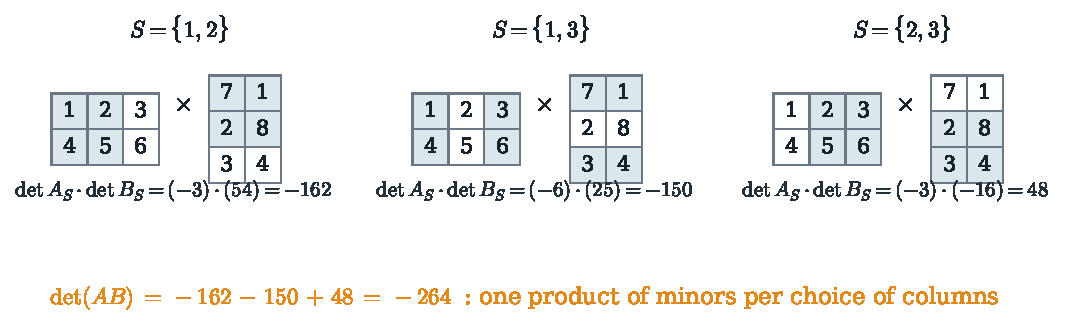
\includegraphics[width=0.98\textwidth]{mt_fig2_cauchybinet}
  \caption{Cauchy--Binet for a $2\times3$ times $3\times2$ product. Three ways to choose two of
  the three middle indices; each contributes the product of the two shaded minors. The three
  products $-162-150+48$ sum to $\det(AB)=-264$, which one checks directly:
  $AB=\left(\begin{smallmatrix}20&29\\56&68\end{smallmatrix}\right)$.}
  \label{fig:cb}
\end{figure}

The Lean proof has three moves, and the middle one is where the formula's content lives.
\emph{First}, expanding $\det(AB)$ by the Leibniz formula and distributing the product over the
matrix-product sums gives an expansion over \emph{all} functions $g:\{1..m\}\to\{1..n\}$,
\[
  \det(AB)\;=\;\sum_{g}\;\det A_{\cdot,g}\cdot\prod_{i}B_{g(i),i}
  \qquad(\lean{det\_mul\_eq\_sum\_submatrix}),
\]
where $A_{\cdot,g}$ repeats columns as $g$ does. \emph{Second}---the heart---fix an injective
image $S$ and sum over the $m!$ relabellings $\pi$ of its columns: the $A$-minor picks up
$\operatorname{sgn}\pi$, and summing the plain products $\prod_i B$ against that sign
\emph{reassembles the determinant of $B_{S,\cdot}$} out of nothing but the Leibniz formula read
backwards (\lean{fiber\_sum}). \emph{Third}, non-injective $g$ die (a repeated column), and the
injective ones biject with pairs (subset, relabelling); Lean's \lean{Finset.sum\_bij} does the
bookkeeping. Nothing here is original mathematics---the proof is essentially Binet's---but the
care in the middle step is what a proof assistant buys: the sign bookkeeping is checked once,
completely, and never again by anyone.

Mathlib does not contain Cauchy--Binet. An independent formalization appeared recently in the
Lean project accompanying Grinberg's textbook~\cite{Grinberg,FaabianRepo}, with a different
architecture; Section~\ref{sec:boundary} compares. The version here is self-contained over a
commutative ring and stated against Mathlib's \lean{Matrix} API, with the sorted-subset
indexing (\lean{Finset.orderEmbOfFin}) that the rest of the chain consumes.

% ---------------------------------------------------------------
\section{The Laplacian is a Gram matrix}
\label{sec:gram}

Mathlib has an incidence matrix, but the unoriented one: a $V\times\mathrm{Sym}^2V$ array of
$0$s and $1$s. Its Gram matrix is $D+A$, the \emph{signless} Laplacian---the wrong sign for
counting trees. The missing object is the \emph{oriented} incidence matrix, and it is the one
place in this development where a definition had to be designed rather than found.

\begin{definition}[{\lean{SimpleGraph.orientedIncMatrix}}]
For a linearly ordered vertex type, let $N\in R^{V\times\mathrm{Sym}^2V}$ have, in the column of
an edge $e=\{u,w\}$ with $u<w$: entry $+1$ at row $w$ (the larger endpoint), $-1$ at row $u$,
and $0$ elsewhere; columns of non-edges are zero.
\end{definition}

Orienting every edge from its smaller to its larger endpoint is arbitrary, and harmlessly so:
any orientation gives the same Gram matrix, because each edge contributes
$(\pm1)^2$ to a diagonal entry and $(+1)(-1)$ to an off-diagonal one. That computation is the
whole proof of:

\begin{theorem}[{\lean{SimpleGraph.orientedIncMatrix\_mul\_transpose}}]
\label{thm:gram}
\keyeq{N\,N^{\mathsf T}\;=\;D-A\;=\;L.}
\end{theorem}

\begin{figure}[t]
  \centering
  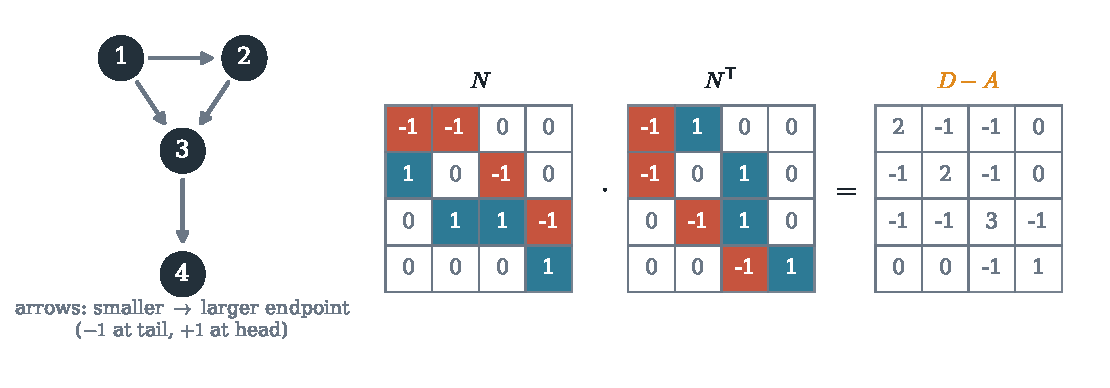
\includegraphics[width=0.98\textwidth]{mt_fig3_gram}
  \caption{Theorem~\ref{thm:gram} on the triangle-with-tail graph. Each column of $N$ holds one
  edge's $\pm1$ pair; row $u$ dotted with itself counts $(\pm1)^2$ once per incident edge (the
  degree), row $u$ dotted with row $w$ sees only the shared edge, contributing $-1$. The signs
  are what make the Laplacian: the unoriented matrix would give $D+A$.}
  \label{fig:gram}
\end{figure}

The utility of the factorization is that it moves spectral facts to bookkeeping: positive
semidefiniteness of $L$ is immediate ($x^{\mathsf T}NN^{\mathsf T}x=\|N^{\mathsf T}x\|^2$ over
$\R$), the kernel is the locally-constant functions, and---the use made here---the determinant
of any square submatrix of $L$ becomes a Cauchy--Binet sum. In Lean the proof is an
entrywise computation: the diagonal squares to the unoriented incidence row
(\lean{orientedIncMatrix\_mul\_self}), whose sum Mathlib already knows is the degree; the
off-diagonal product of two distinct rows is supported on their common edge, where the signs are
opposite by construction.

% ---------------------------------------------------------------
\section{Delete a root, square the minors}
\label{sec:sum}

The Laplacian itself is singular, so the count lives one deletion down. Fix the root $v_0$;
write $N_0$ for $N$ without the row of $v_0$, and $L_0$ for $L$ without the row and column of
$v_0$. Restricting Theorem~\ref{thm:gram} gives $L_0=N_0N_0^{\mathsf T}$, and now $N_0$ is an
$(n-1)\times\binom{|V|}{2}$ rectangle: exactly Cauchy--Binet's shape, with $B=N_0^{\mathsf T}$
the transpose of $A=N_0$, so each summand is a product of a minor with its own transpose---a
square.

\begin{theorem}[{\lean{SimpleGraph.det\_reducedLapMatrix\_eq\_sum\_sq}}]
\label{thm:sum}
\keyeq{\det L_0\;=\;\sum_{\substack{S\subseteq\mathrm{Sym}^2V\\ |S|=n-1}}
  \bigl(\det N_{0,S}\bigr)^{2}}
where $N_{0,S}$ is the square minor of $N_0$ on the columns $S$.
\end{theorem}

Note where the sum ranges: over \emph{all} $(n-1)$-subsets of vertex pairs, edges or not. The
columns of non-edges are zero, so their subsets contribute nothing---but they are honestly in
the sum, and the formal statement says so. For $K_4$ the sum has $\binom{6}{3}=20$ terms;
Table~\ref{tab:k4} classifies them. The determinant has become a \emph{census}: the rest of the
proof is deciding, subset by subset, who contributes.

\begin{table}[h]
\centering
\rowcolors{2}{ggband!35}{white}
\begin{tabular}{lccc}
\toprule
\rowcolor{ggteal!18} the 20 subsets ($K_4$, $|S|=3$) & how many & $(\det N_{0,S})^2$ & contribution \\
\midrule
spanning trees                  & 16 & 1 & 16 \\
triangles (4th vertex isolated) & 4  & 0 & 0  \\
\bottomrule
\end{tabular}
\caption{The census for $K_4$: every 3-subset of its 6 edges either spans a tree or is one of
the four triangles, which leave a vertex stranded. $\det L_0=16+0=16$, matching
Figure~\ref{fig:k4}. (A 3-subset of edges on 4 vertices fails to be a spanning tree exactly
when it is a triangle.)}
\label{tab:k4}
\end{table}

One technical remark, since it is the kind a formalization cannot wave away: Cauchy--Binet
needs a linear order on the column type $\mathrm{Sym}^2V$ to name its sorted minors. None is
canonical, so the development installs a scoped one---lexicographic on the (smaller, larger)
endpoint pair---purely as indexing apparatus. Determinants squared do not care which order was
chosen, and the statement of Theorem~\ref{thm:sum} quantifies over subsets, not orderings.

% ---------------------------------------------------------------
\section{Which minors survive: sorting instead of inducting}
\label{sec:dichotomy}

\begin{theorem}[{\lean{SimpleGraph.sq\_det\_minor\_eq\_ite}}]
\label{thm:dichotomy}
Let $R$ be an integral domain and $|S|=n-1$. Then
\keyeq{\bigl(\det N_{0,S}\bigr)^2\;=\;
\begin{cases}
  1 & \text{if } S\subseteq E(G)\ \text{and}\ (V,S)\ \text{is connected,}\\[2pt]
  0 & \text{otherwise.}
\end{cases}}
\end{theorem}

With $n-1$ edges, ``connected'' \emph{is} ``spanning tree''; the Lean statement uses the
connectivity form because that is what the proof consumes, and a separate lemma converts it to
\lean{IsTree} for the headline (\lean{connected\_fromEdgeSet\_iff\_isTree}). The proof is
three cases, in increasing order of interest.

\emph{A non-edge in $S$.} Its column of $N_0$ is zero, and a determinant with a zero column is
zero. This is also where the diagonal of $\mathrm{Sym}^2V$ goes: a loop $\{v,v\}$ is not an edge
of a simple graph, so subsets containing one die here too.

\emph{All edges, but $(V,S)$ disconnected.} Some connected component $C$ misses the root.
Add up the rows of $N_{0,S}$ over the vertices of $C$: each column of an edge inside $C$ meets
both its $+1$ and its $-1$; no edge of $S$ leaves $C$; the result is the zero row vector,
exhibited in Lean as a nonzero kernel vector of the transpose
(\lean{Matrix.exists\_vecMul\_eq\_zero\_iff}---this is the one step that wants an integral
domain). For the failing subsets of Table~\ref{tab:k4} the component is a single stranded
vertex, and the dependence is just ``its row is zero''; in general $C$ can be larger, and the
indicator vector of $C$ does the work.

\emph{All edges, $(V,S)$ connected.} This is the case the textbooks prove by peeling a leaf and
inducting on $n$, and the case where the formal proof does something different.

\begin{figure}[t]
  \centering
  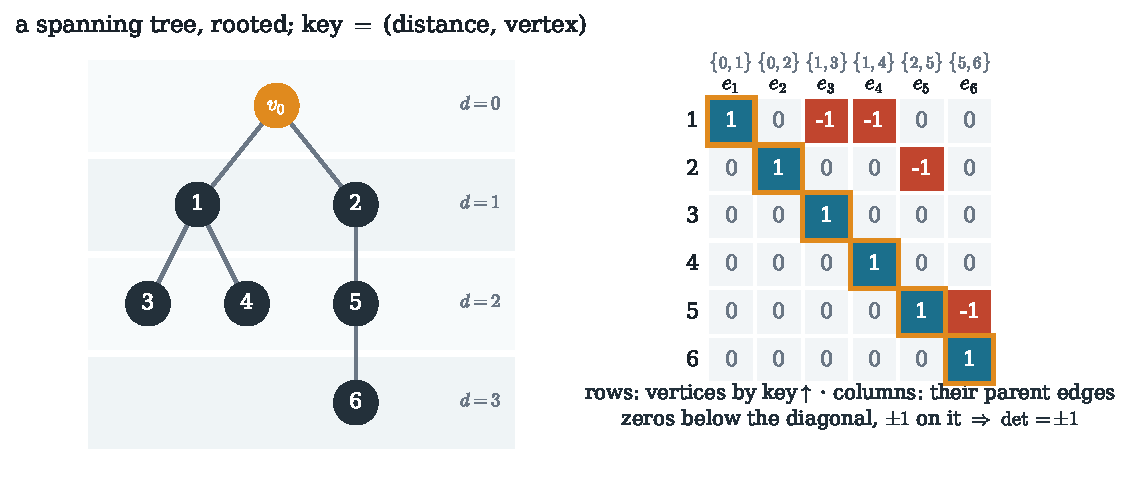
\includegraphics[width=0.97\textwidth]{mt_fig4_triangular}
  \caption{The connected case of Theorem~\ref{thm:dichotomy}. Left: a spanning tree rooted at
  $v_0$, vertices keyed by (distance to root, vertex). Right: the minor $N_{0,S}$ with each
  vertex's column chosen as its \emph{parent edge} and both sides sorted by the key. A vertex
  meets its own parent edge on the diagonal ($\pm1$, framed) and its children's parent edges to
  the right (their key is larger); everything below the diagonal vanishes, so
  $\det=\pm1$ by reading the diagonal.}
  \label{fig:triangular}
\end{figure}

Every non-root vertex $u$ of a connected subgraph has a neighbour strictly closer to the root:
the second vertex of any geodesic from $u$ to $v_0$. Call the edge to that neighbour the
\emph{parent edge} of $u$. Two facts, both proved by distance arithmetic alone:

\begin{itemize}
\item \emph{The map $u\mapsto\text{parent edge of }u$ is injective.} If two vertices shared a
parent edge in the swapped way ($u$ the parent of $u'$ and $u'$ of $u$), their distances to the
root would satisfy $d(u)=d(u)+2$. With $|S|=n-1$ and $n-1$ non-root vertices, injective means
bijective: \emph{every} edge of $S$ is somebody's parent edge.
\item \emph{Triangularity.} Recolumn the minor so that vertex $u$'s column is its parent edge,
and sort rows and columns by the key $(\dist(u,v_0),u)$. A nonzero entry in row $u$, column
(parent edge of $w$) forces $u\in\{w,\text{parent of }w\}$: either the diagonal, or
$\dist(u,v_0)=\dist(w,v_0)-1$, strictly \emph{smaller} key. Everything below the diagonal is
zero (Figure~\ref{fig:triangular}), the diagonal entries are $\pm1$ (each vertex sits on its own
parent edge), and $\det N_{0,S}=\pm1$.
\end{itemize}

In Lean the recolumning is an \lean{Equiv} built from injectivity plus the cardinality count,
the sorting is \lean{Finset.orderIsoOfFin} applied to the image of the key, the vanishing is
\lean{Matrix.BlockTriangular} with \lean{Matrix.det\_of\_upperTriangular}, and the sign washes
out in the square. Two engineering choices are worth naming plainly. \emph{No induction}: the
linear order on keys does the work that leaf-deletion recursion does in the textbook proof, and
a sorted matrix is something a proof assistant handles far more gracefully than a graph
surgery. \emph{No separate acyclicity lemma}: connectivity gives every vertex a parent and the
count makes the parent map onto, which is all the argument needs. Mathematically this is no
surprise---with $n-1$ edges, connectivity and acyclicity are equivalent characterizations of
the same trees---but in a formal development the choice of which characterization to consume is
real work saved, and here the acyclic half never has to be materialized.

% ---------------------------------------------------------------
\section{Numerical verification}
\label{sec:verification}

Each link of the chain was validated numerically---in exact arithmetic, never
floating-point---\emph{before} its Lean proof was attempted, and the assembled statement was
validated end-to-end afterwards. Table~\ref{tab:verification} summarizes.

\begin{table}[h]
\centering\small
\rowcolors{2}{ggband!35}{white}
\begin{tabular}{lll}
\toprule
\rowcolor{ggteal!18} check & scope & result \\
\midrule
Cauchy--Binet statement, sorted-subset indexing & $2\times3\cdot3\times2$, exact & match ($-264$) \\
tree minors: triangular under the key, $\det=\pm1$ & 200 random trees, $n\le9$ & all pass \\
non-tree $(n{-}1)$-edge subsets: $\det=0$ & 158 random graphs & all pass \\
$(\det N_{0,S})^2=\mathbb 1[S$ spans a tree$]$, every $S$ & 40 random graphs, all $S$ & all pass \\
$\sum_S(\det N_{0,S})^2=\det L_0=\tau(G)$ & same 40 graphs & all pass \\
named graphs (Table~\ref{tab:numbers}) & 6 graphs & all match \\
\lean{\#print axioms}, all five theorems & --- & 3 standard axioms \\
full library build & \lean{lake build} & 3074 jobs, no errors \\
\bottomrule
\end{tabular}
\caption{The verification battery (SageMath 10, exact integer arithmetic).}
\label{tab:verification}
\end{table}

\emph{Size and dependencies.} The development is small: $834$ lines of Lean across the five
files of Table~\ref{tab:loadbearing}, containing $35$ declarations in total ($28$ theorems and
lemmas, six definitions, one scoped instance), importing eleven Mathlib files (the
\lean{SimpleGraph} core, \lean{LapMatrix}, \lean{IncMatrix}, the graph metric, the determinant
and block-triangular API, and \lean{Sym2} ordering). Against a warm Mathlib v4.30 cache each
file rechecks in $7$--$9$ seconds; the full project build (library and all parts of the series)
is $3074$ jobs.

One incident from this battery is worth reporting, because it shows the method earning its keep.
The first numerical model of the minor placed $\pm1$ entries in \emph{every} column, non-edges
included, and promptly produced a counterexample to Theorem~\ref{thm:dichotomy}: a spanning
star whose edges did not all belong to the graph still had $\det=\pm1$. The discrepancy was in
the model, not the mathematics---the Lean \lean{orientedIncMatrix} gives non-edges \emph{zero}
columns, which is precisely case one of the dichotomy---and the corrected model passed all
$40$ graphs. A verification harness that cannot catch its operator's own mistakes is
decoration; this one caught mine.

% ---------------------------------------------------------------
\section{The boundary: what is proved and what is not}
\label{sec:boundary}

\emph{Proved.} Theorems~\ref{thm:cb}--\ref{thm:kirchhoff}, \lean{sorry}-free, for finite simple
graphs, any root, over any integral domain ($\Z$, $\mathbb Q$, $\R$, \dots). The five
\lean{\#print axioms} calls report \lean{propext}, \lean{Classical.choice}, \lean{Quot.sound}
and nothing else.

\emph{The domain hypothesis.} Cases one and three of the dichotomy hold over any commutative
ring; the disconnected case turns a kernel vector into a vanishing determinant, which is where
zero divisors would interfere. Since the headline equality is between a determinant and a
natural number, proving it over $\Z$ (or $\mathbb Q$) and transporting is no loss; the
hypothesis is stated honestly rather than hidden.

\emph{Counting, not constructing.} The proof is noncomputable in Lean's sense: parents are
chosen with \lean{Classical.choice}, and no algorithm (for counting or for sampling) is
extracted. The determinant on the left is, of course, computable by any linear-algebra system;
the theorem is what \emph{justifies} that computation.

\emph{Not built, mapped.} The weighted version (the Kirchhoff polynomial: give each edge an
indeterminate and the reduced determinant enumerates trees by monomials) needs only the same
chain with weighted $\pm$ entries---the dichotomy's triangular argument goes through with
$x_e$ in place of $\pm1$---but it is not formalized here. Likewise the all-minors
theorem~\cite{ChaikenKleitman1978}, the directed/arborescence version~\cite{Tutte1948}, and the
$\det L_0$-independence-of-root as a standalone statement (here it is a corollary: both sides
count the same trees).

\emph{Prior art, stated exactly.} For Cauchy--Binet: Mathlib has no version and, at the time of
writing, no pull request mentioning it; an independent Lean formalization exists in the
project formalizing Grinberg's \emph{An Introduction to Algebraic
Combinatorics}~\cite{Grinberg,FaabianRepo}, with a different proof architecture (explicit
permutation extraction/reconstruction, where this development sums fibers and lets the
$B$-determinant reassemble itself). That project predates this one; the version here is
independent and was built for the chain above. For the matrix-tree theorem itself I searched
the Lean ecosystem, the Isabelle Archive of Formal Proofs, and the Coq/Rocq corpus, and was
unable to locate one; to the best of my knowledge there is none, and I would welcome a
correction.

% ---------------------------------------------------------------
\section{Implications and methodology}
\label{sec:implications}

\emph{Where the theorem goes to work.} Three consumers, each with the exact quantity the
theorem supplies. \emph{Network reliability}: $\tau(G)$ is the all-terminal reliability
polynomial's leading combinatorial datum; comparing designs means comparing spanning-tree
counts, and Table~\ref{tab:numbers} is how one computes them. \emph{Random spanning trees}:
Wilson's algorithm~\cite{Wilson1996} samples uniformly among $\tau(G)$ trees; the
transfer-current theorem~\cite{BurtonPemantle1993} makes edge-membership probabilities
determinantal---ratios $\tau(G/e)/\tau(G)$ of tree counts, i.e.\ effective resistances.
\emph{Spectral sparsification}: sampling edges by effective resistance approximately preserves
the Laplacian quadratic form, with high probability~\cite{SpielmanSrivastava2011}; the quantity being sampled by is, again, a ratio of the
two sides of this theorem. None of these pipelines is formalized here; what is formalized is the
identity they all stand on.

\emph{For the library.} Two pieces are natural Mathlib candidates independently of Kirchhoff:
Cauchy--Binet (Section~\ref{sec:cb}), and the oriented incidence matrix with its factorization
$NN^{\mathsf T}=D-A$ (Section~\ref{sec:gram}), which complements the existing unoriented
\lean{incMatrix} and its $D+A$. The dichotomy argument also isolates a reusable pattern:
\emph{replace structural induction by a sort}---find the right injective key, and
\lean{BlockTriangular} turns a graph-theoretic recursion into one determinant read-off.

\emph{Methodology.} As in Parts~I--IV, the formalization was carried out with an AI assistant
(Claude, Anthropic) operating Lean against a local Mathlib; the human author set the direction,
audited every claim, and is responsible for every statement. The working rules are unchanged
and brief: ``proven'' means \lean{sorry}-free with axioms printed; designs are de-risked
numerically in exact arithmetic before formalization (Section~\ref{sec:verification}); novelty
claims are checked against the literature and the other proof-assistant ecosystems, and prior
work found---here, the independent Cauchy--Binet of~\cite{FaabianRepo}---is reported rather
than elided.

% ---------------------------------------------------------------
\section{Questions left open}
\label{sec:questions}

A formalization is also a list of the next questions, sharpened until a machine could be asked
them.

\begin{itemize}
\item The triangular argument reads $\det N_{0,S}=\pm1$ off a sorted diagonal. The
\emph{weighted} minor, with indeterminate $x_e$ in place of $\pm1$, is triangular by the same
key, with diagonal $\pm\prod_{e\in S}$\,(one weight per parent edge). Does the identical proof
skeleton yield the Kirchhoff polynomial $\sum_T\prod_{e\in T}x_e$ with only the diagonal
read-off changed---and if so, is the weighted statement the \emph{right} Mathlib-level
generality from the start?
\item The disconnected case needs an integral domain to turn a kernel vector into
$\det=0$. The determinant of a matrix with a rootless component is in fact zero over \emph{any}
commutative ring (it is an integer identity). Can the dichotomy be proved ring-generically,
e.g.\ by exhibiting the vanishing as a polynomial identity in the entries, and the domain
hypothesis dropped from Theorem~\ref{thm:kirchhoff}?
\item ``Sorting instead of inducting'' worked because the parent map plus a linear key made the
minor triangular. Which other graph inductions are secretly sorts? The all-minors
theorem~\cite{ChaikenKleitman1978} replaces trees by rooted forests---is there a multi-root key
that triangularizes those minors in one pass?
\item Both this paper and Part~IV ended with a determinant identity whose proof never touches
the combinatorial object it counts (there, closed walks; here, cycles). Is there a common
formal interface---``count by triangularizing a Gram minor''---under which the matching-side
and tree-side determinants become instances of one lemma?
\item Mathlib's \lean{Matrix.TotallyUnimodular} is exactly the predicate ``every square minor
is $0$ or $\pm1$''. The dichotomy establishes this for the \emph{maximal} minors of the reduced
matrix $N_0$; the classical fact is that oriented incidence matrices are totally unimodular,
all orders included. Would proving and registering full total unimodularity connect this
development to the optimization-flavoured part of the library, and does the parent-edge
argument extend below the top order?
\end{itemize}

And one to keep. \emph{Kirchhoff wanted currents, and the determinant handed him the trees he
had not asked for; the proof above never once looks at a cycle, yet ends knowing exactly how
many ways the graph avoids them all. How much else does a library that can take determinants
already know, and simply not yet say?}

% ---------------------------------------------------------------
\begin{thebibliography}{99}

% --- the two memoirs of 1812 ---
\bibitem{Binet1812} J.~P.~M. Binet, \emph{M\'emoire sur un syst\`eme de formules analytiques,
et leur application \`a des consid\'erations g\'eom\'etriques}, J.~\'Ec.\ Polytech.\
\textbf{9}, cahier~16 (1813). Read 30 November 1812.
\bibitem{Cauchy1812} A.-L. Cauchy, \emph{M\'emoire sur les fonctions qui ne peuvent obtenir que
deux valeurs \'egales et de signes contraires par suite des transpositions op\'er\'ees entre
les variables qu'elles renferment}, J.~\'Ec.\ Polytech.\ \textbf{10}, cahier~17 (1815),
29--112. Read 30 November 1812.

% --- the matrix-tree theorem: origin and classical proofs ---
\bibitem{Kirchhoff1847} G.~Kirchhoff, \emph{\"Uber die Aufl\"osung der Gleichungen, auf welche
man bei der Untersuchung der linearen Vertheilung galvanischer Str\"ome gef\"uhrt wird},
Ann.\ Phys.\ Chem.\ \textbf{72} (1847), 497--508.
\bibitem{Borchardt1860} C.~W. Borchardt, \emph{\"Uber eine Interpolationsformel f\"ur eine Art
symmetrischer Functionen und \"uber deren Anwendung}, Abh.\ K\"onigl.\ Akad.\ Wiss.\ Berlin
(1860), 1--20.
\bibitem{Cayley1889} A.~Cayley, \emph{A theorem on trees}, Quart.\ J.~Pure Appl.\ Math.\
\textbf{23} (1889), 376--378.
\bibitem{BSST1940} R.~L. Brooks, C.~A.~B. Smith, A.~H. Stone, and W.~T. Tutte, \emph{The
dissection of rectangles into squares}, Duke Math.\ J.~\textbf{7} (1940), 312--340.
\bibitem{Tutte1948} W.~T. Tutte, \emph{The dissection of equilateral triangles into equilateral
triangles}, Proc.\ Cambridge Philos.\ Soc.\ \textbf{44} (1948), 463--482.
\bibitem{ChaikenKleitman1978} S.~Chaiken and D.~J. Kleitman, \emph{Matrix tree theorems},
J.~Combin.\ Theory Ser.~A \textbf{24} (1978), 377--381.
\bibitem{Chaiken1982} S.~Chaiken, \emph{A combinatorial proof of the all minors matrix tree
theorem}, SIAM J.~Algebraic Discrete Methods \textbf{3} (1982), 319--329.

% --- standard accounts ---
\bibitem{Moon1970} J.~W. Moon, \emph{Counting Labelled Trees}, Canadian Math.\ Monographs
\textbf{1}, Canadian Math.\ Congress, 1970.
\bibitem{Biggs1993} N.~Biggs, \emph{Algebraic Graph Theory}, 2nd ed., Cambridge Univ.\ Press,
1993.
\bibitem{GodsilRoyle} C.~Godsil and G.~Royle, \emph{Algebraic Graph Theory}, Grad.\ Texts in
Math.\ \textbf{207}, Springer, 2001.
\bibitem{StanleyEC2} R.~P. Stanley, \emph{Enumerative Combinatorics, Volume~2}, Cambridge
Stud.\ Adv.\ Math.\ \textbf{62}, Cambridge Univ.\ Press, 1999.

% --- modern probability and algorithms on spanning trees ---
\bibitem{Wilson1996} D.~B. Wilson, \emph{Generating random spanning trees more quickly than the
cover time}, in \emph{Proc.\ 28th ACM Symp.\ Theory of Computing} (STOC~1996), 296--303.
\bibitem{BurtonPemantle1993} R.~Burton and R.~Pemantle, \emph{Local characteristics, entropy
and limit theorems for spanning trees and domino tilings via transfer-impedances}, Ann.\
Probab.\ \textbf{21} (1993), 1329--1371.
\bibitem{SpielmanSrivastava2011} D.~A. Spielman and N.~Srivastava, \emph{Graph sparsification
by effective resistances}, SIAM J.~Comput.\ \textbf{40} (2011), 1913--1926.
\bibitem{LyonsPeres} R.~Lyons and Y.~Peres, \emph{Probability on Trees and Networks}, Cambridge
Univ.\ Press, 2016.

% --- formalization context ---
\bibitem{Grinberg} D.~Grinberg, \emph{An Introduction to Algebraic Combinatorics}, lecture
notes, 2026. \texttt{arXiv:2506.00738}.
\bibitem{FaabianRepo} \emph{algebraic-combinatorics: a Lean~4 formalization of Grinberg's ``An
Introduction to Algebraic Combinatorics''},
\url{https://github.com/faabian/algebraic-combinatorics}, 2026. Cauchy--Binet in blueprint
\S5.2.
\bibitem{Mathlib} The mathlib Community, \emph{The Lean mathematical library}, in \emph{Proc.\
9th ACM SIGPLAN Int.\ Conf.\ on Certified Programs and Proofs} (CPP~2020), 367--381.

% --- this series ---
\bibitem{PartI} C.~Mar\'in, \emph{Random Signs into Matchings: the Godsil--Gutman estimator and
real-rootedness in Lean~4} (Part~I), 2026. Zenodo, DOI \texttt{10.5281/zenodo.20517350}.
\bibitem{PartII} C.~Mar\'in, \emph{Unfolding a Graph into a Tree: A Machine-Checked Proof of
the Heilmann--Lieb Theorem in Lean~4} (Part~II), 2026. Zenodo, DOI
\texttt{10.5281/zenodo.20561832}.
\bibitem{Bass} C.~Mar\'in, \emph{Folding Edges into Vertices: A Machine-Checked Proof of Bass's
Determinant Formula for the Ihara Zeta in Lean~4}, 2026. Zenodo, DOI
\texttt{10.5281/zenodo.20573120}.
\bibitem{PartIII} C.~Mar\'in, \emph{Walks that Forget the Cycles: A Machine-Checked Bijection
between Tree-Like Walks of a Graph and Walks on Godsil's Path Tree, in Lean~4} (Part~III),
2026. Zenodo, DOI \texttt{10.5281/zenodo.20600326}.
\bibitem{PartIV} C.~Mar\'in, \emph{When Walks Become a Spectrum: A Machine-Checked Proof of
Godsil's Moment Theorem in Lean~4} (Part~IV), 2026. Zenodo, DOI
\texttt{10.5281/zenodo.20613247}.

\end{thebibliography}

\end{document}
